% !TEX program = xelatex
\documentclass[]{article}
\usepackage{commons/course}

\begin{document}
\printheader

\section*{سوال اول}
\subsection*{قسمت اول}
\begin{gather*}
    S \rightarrow 0S0 | 0S1 | 1S0 | 1S1 | 0
\end{gather*}
\subsection*{قسمت دوم}
\begin{gather*}
    S \rightarrow 0S0 | 1S1 | \epsilon
\end{gather*}
\subsection*{قسمت سوم}
عبارت
$R_i$
یعنی اینکه به
$i$
0 دیگر نیاز داریم
که شرط مسئله ارضا شود.
\begin{align*}
    S &\rightarrow R_3\\
    R_3 &\rightarrow 1R_3 | 0R_2\\
    R_2 &\rightarrow 1R_2 | 0R_1\\
    R_1 &\rightarrow 1R_1 | 0R_0\\
    R_0 &\rightarrow 1R_0 | 0R_0 | \epsilon\\
\end{align*}
\section*{سوال دوم}
\begin{enumerate}
    \item رشته‌هایی که طول آن‌ها فرد است.
    \item $1^a 0^b, \quad a, b \ge 0$
\end{enumerate}
\section*{سوال سوم}
\subsection*{قسمت اول}
برای اینکه مورد خواسته شده در سوال را چک کنیم کافی است برای هر قانون در گرامر شرط‌های زیر را چک
بکنیم: به ازای هر قانون
$A \rightarrow \alpha | \beta$
باید:
\begin{enumerate}
    \item $\operatorname{First}(\alpha) \cap \operatorname{First}(\beta) = \emptyset$
    \item در صورتی که $\alpha \implies^* \epsilon$ آنگاه  $\operatorname{Follow}(\alpha) \cap \operatorname{First}(\beta) = \emptyset$
    \item فقط یکی از عبارت $\alpha \implies^* \epsilon$ و $\beta \implies^* \epsilon$ درست است.
\end{enumerate}
پس در ابتدا
\lr{First}
تمامی
\lr{non terminal}ها
را پیدا می‌کنیم. (مشخص است که \lr{First} همه‌ی \lr{terminal}ها خودشان هستند.)
\begin{align*}
    \operatorname{First}(S) &= \{a\}\\
    \operatorname{First}(A) &= \{a, b\}\\
    \operatorname{First}(B) &= \{\epsilon, a, b\}\\
    \operatorname{First}(C) &= \{b, a\}\\
    \operatorname{First}(D) &= \{d\}
\end{align*}
اما در همان قاعده‌ی اول به مشکل می‌خوریم. چرا که
$\operatorname{First}(aaB)$ و $\operatorname{First}(aAC)$
هر جفتشان
$a$
هستند و در نتیجه نمی‌توان که پیش بینی کرد که باید کدام قاعده را باز کرد.
\subsection*{قسمت دوم}
در ابتدا از قاعده‌ی آخر شروع می‌کنیم که کلا قاعده‌ی اضافی است و هیچ‌جایی استفاده نمی‌شود.
این قاعده عملا زبان
$d^n$
است که پس می‌توان صرفا آن را به صورت
$D \rightarrow dD', D' \rightarrow dD' | \epsilon$
نوشت. حال نکته‌ای که باید به آن توجه بکنید این است که بقیه‌ی قاعده‌ها
\lr{left recursion}
ندارند. حتی اگر قاعده‌ها را دنبال نیز بکنیم باز هم به هیچ
\lr{let recursion}ای
نمی‌رسیم چرا که از سمت چپ نمی‌توان یک
\lr{loop}
زد در
\lr{non terminal}ها.
حال با این موضوع سعی می‌کنیم که با فاکتورگیری از گرامر آن را
predictive
کنیم. در ابتدا دقت کنید که در قانون دوم هر دو طرف می‌توانند که با
$a$
شروع شوند. چرا که می‌توان
$B$ را به $C$ برد و $C$ را به $abc$.
پس عملا با بازنوسی داریم:
\begin{gather*}
    A \rightarrow abcCbCbC | bCbCbC | bC | a
\end{gather*}
پس در اینجا
$a$ و $b$
را فاکتور می‌گیریم.
\begin{align*}
    A  &\rightarrow aA' | bCA''\\
    A' &\rightarrow bcCbCbC | \epsilon\\
    A'' &\rightarrow bCbC | \epsilon
\end{align*}
همان طور که مشاهده می‌شود حال سمت راست قواعد درست شده قابل
\lr{prediction}
هستند. حال سراغ قاعده‌ی
$S$
می‌رویم و
$a$
را فاکتور می‌گیریم.
\begin{align*}
    S &\rightarrow aS'\\
    S' &\rightarrow aB | AC
\end{align*}
اما هنوز کار ما تمام نشده است چرا که
$\operatorname{First}(aB)$ و $\operatorname{First}(AC)$
هر دو
$a$
دارند. در ابتدا دقت کنید که
$S' \rightarrow aB | aA'C | bCA''C$
پس کافی است که یک فاکتور گیری دیگر از
$a$
داشته باشیم:
\begin{align*}
    S &\rightarrow aS'\\
    S' &\rightarrow aS'' | bCA''C\\
    S'' &\rightarrow B | A'C
\end{align*}
حال
$B$ و $A'$
را باز می‌کنیم:
\begin{gather*}
    S'' \rightarrow CCbC | bcCbCbCC | C | \epsilon
\end{gather*}
در نهایت می‌توان
$S''$
را به صورت زیر نوشت:
\begin{align*}
    S'' &\rightarrow abcCbC | bCbC | bcCbCbCC | abc | b | \epsilon\\
    &\implies\\
    S'' &\rightarrow abcS''' | bS'''' | \epsilon\\
    S''' &\rightarrow CbC | \epsilon\\
    S'''' &\rightarrow CbC | cCbCbCC | \epsilon
\end{align*}
پس در نهایت قوانین ما برابر هستند با:
\begin{align*}
    S &\rightarrow aS'\\
    S' &\rightarrow aS'' | bCA''C\\
    S'' &\rightarrow abcS''' | bS'''' | \epsilon\\
    S''' &\rightarrow CbC | \epsilon\\
    S'''' &\rightarrow CbC | cCbCbCC | \epsilon\\
    A  &\rightarrow aA' | bCA''\\
    A' &\rightarrow bcCbCbC | \epsilon\\
    A'' &\rightarrow bCbC | \epsilon\\
    B &\rightarrow CCbC | \epsilon\\
    C &\rightarrow abc | b\\
    D &\rightarrow dD'\\
    D' &\rightarrow dD' | \epsilon
\end{align*}
\section*{سوال چهارم}
در ابتدا خود قوانین را به صورت ریاضی می‌نویسیم:
\begin{align*}
    S &\rightarrow MN\\
    M &\rightarrow mN | \epsilon\\
    N &\rightarrow OPQ\\
    O &\rightarrow nO | \epsilon\\
    P &\rightarrow pP | \epsilon\\
    Q &\rightarrow qQ | \epsilon
\end{align*}
در ابتدا مشخص است که کلا
\lr{left recursion}
کلا نداریم. حال همان طور که سوال خواسته هست
\lr{First} و \lr{Follow}
هر یک از علامت‌ها را بدست می‌آوریم. دقت کنید که
\lr{First}
هر پایانه خودش است پس آن‌ها را اصلا نمی‌نویسیم.
\begin{align*}
    \operatorname{First}(Q) &= \{q, \epsilon\}\\
    \operatorname{First}(P) &= \{p, \epsilon\}\\
    \operatorname{First}(O) &= \{n, \epsilon\}\\
    \operatorname{First}(N) &= \{n, p, q, \epsilon\}\\
    \operatorname{First}(M) &= \{m, \epsilon\}\\
    \operatorname{First}(S) &= \{m, n, p, q, \epsilon\}\\
    \operatorname{Follow}(S) &= \{\$\}\\
    \operatorname{Follow}(M) &= \{n, p, q, \$\}\\
    \operatorname{Follow}(N) &= \{n, p, q, \$\}\\
    \operatorname{Follow}(O) &= \{n, p, q, \$\}\\
    \operatorname{Follow}(P) &= \{n, p, q, \$\}\\
    \operatorname{Follow}(Q) &= \{n, p, q, \$\}
\end{align*}
در ادامه جدول
\lr{LL(1)}
را رسم می‌کنیم. دقت کنید که ترمینال
$o$
کلا جایی استفاده نشده بود برای همین ستونش خالی است.
\begin{latin}
    \centering
    \begin{tabular}{|c|c|c|c|c|c|c|c|}
        \hline
        & \textbf{m} & \textbf{n} & \textbf{o} & \textbf{p} & \textbf{q} & \textbf{\$}\\
        \hline
        \textbf{S} & MN & MN && MN & MN & MN\\
        \hline
        \textbf{M} & mN & $\epsilon$ &&$\epsilon$&$\epsilon$&$\epsilon$\\
        \hline
        \textbf{N} &&OPQ&&OPQ&OPQ&OPQ\\
        \hline
        \textbf{O} &&nO&&$\epsilon$&$\epsilon$&$\epsilon$\\
        \hline
        \textbf{P} &&$\epsilon$&&pP&$\epsilon$&$\epsilon$\\
        \hline
        \textbf{Q} &&$\epsilon$&&$\epsilon$&qQ&$\epsilon$\\
        \hline
    \end{tabular}
\end{latin}
حال برای پارس کردن از سه ستون استفاده می‌کنیم که پشته و ورودی خوانده نشده و عملی که قرار است انجام بدهیم
را دارا است.
\begin{latin}
    \centering
    \begin{tabular}{c|c|c}
        \textbf{Stack} & \textbf{Buffer} & \textbf{Action}\\
        \hline
        S\$ & mnmnpqq\$ & MN\\
        MN\$ & mnmnpqq\$ & mM\\
        mMN\$ & mnmnpqq\$ & terminal\\
        MN\$ & nmnpqq\$ & $\epsilon$\\
        N\$ & nmnpqq\$ & OPQ\\
        OPQ\$ & nmnpqq\$ & nO\\
        nOPQ\$ & nmnpqq\$ & terminal\\
        OPQ\$ & mnpqq\$ & ERROR! SKIP UNITL $\{n, p, q, \$\}$\\
        OPQ\$ & npqq\$ & nO\\
        OPQ\$ & pqq\$ & terminal\\
        PQ\$ & pqq\$ & $\epsilon$\\
        PQ\$ & pqq\$ & pP\\
        pPQ\$ & pqq\$ & terminal\\
        PQ\$ & qq\$ & $\epsilon$\\
        Q\$ & qq\$ & qQ\\
        qQ\$ & qq\$ & terminal\\
        Q\$ & q\$ & qQ\\
        qQ\$ & q\$ & terminal\\
        Q\$ & \$ & $\epsilon$\\
        \$ & \$ & ACCEPT\\
    \end{tabular}
\end{latin}
\section*{سوال پنجم}
\subsection*{قسمت اول}
در ابتدا باید
\lr{left recursion}
را حذف کنیم. پس قوانین ما برابر می‌شوند با:
\begin{align*}
    A &\rightarrow B | B + A | B - A\\
    B &\rightarrow C | C * B | C / B\\
    C &\rightarrow \text{num} \, C' | \text{id} \, C'\\
    C' &\rightarrow \epsilon | *
\end{align*}
\begin{figure}[H]
    \centering
    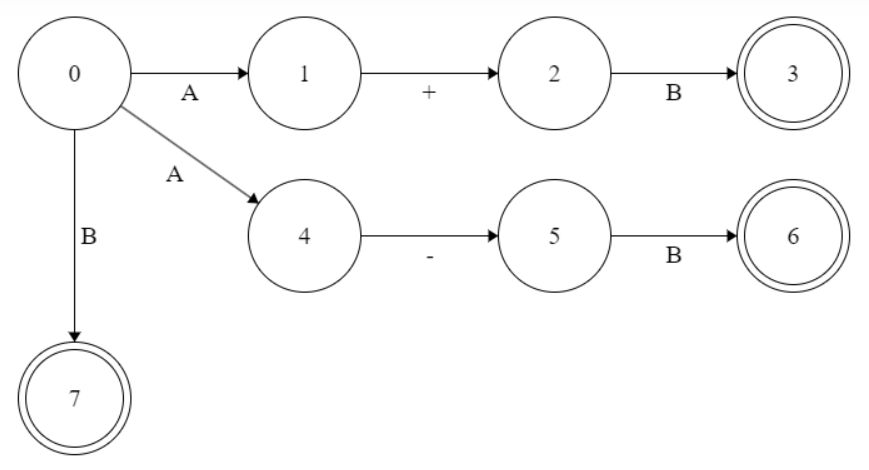
\includegraphics[scale=0.5]{figure/5-1-A.png}
    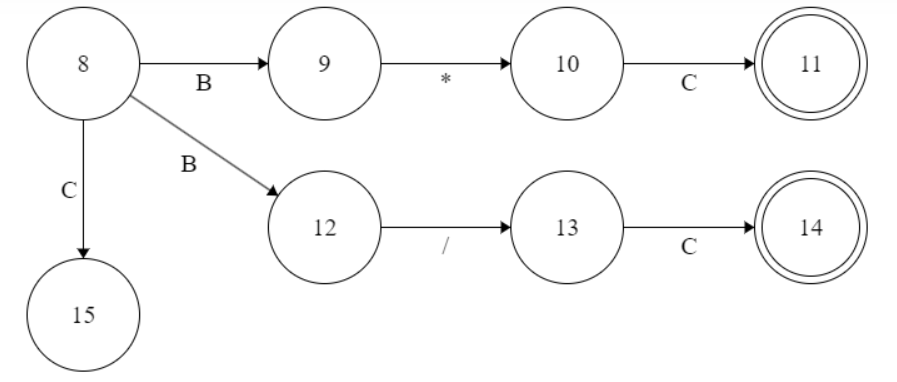
\includegraphics[scale=0.5]{figure/5-1-B.png}
    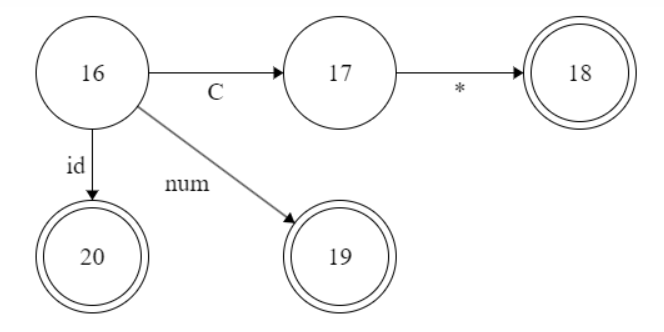
\includegraphics[scale=0.5]{figure/5-1-C.png}
\end{figure}
حال برای ساده سازی هم در ابتدا سعی می‌کنیم حالات تکراری را حذف کنیم.
\begin{figure}[H]
    \centering
    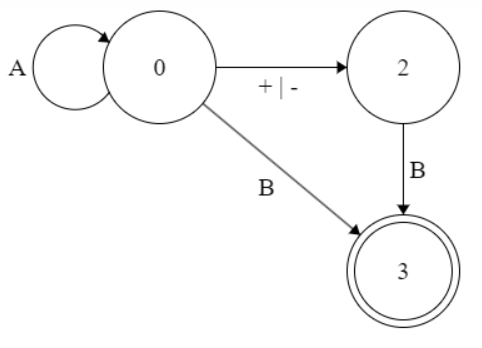
\includegraphics[scale=0.5]{figure/5-1-A-2.png}
    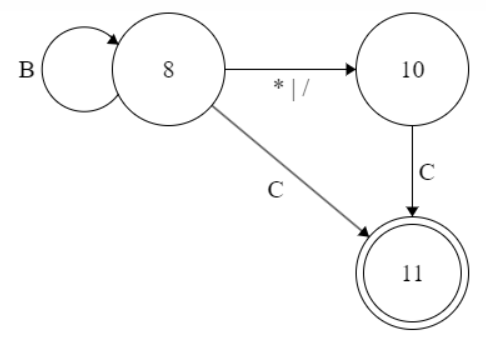
\includegraphics[scale=0.5]{figure/5-1-B-2.png}
    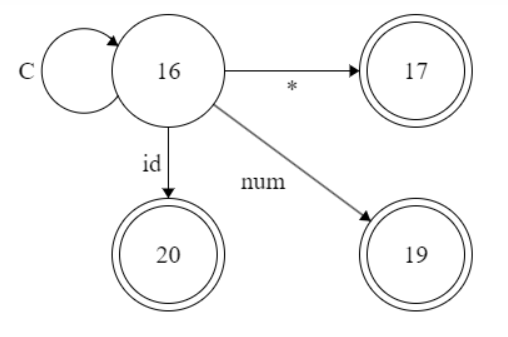
\includegraphics[scale=0.5]{figure/5-1-C-2.png}
\end{figure}
\subsection*{قسمت دوم}
در ابتدا بدون ساده سازی تمامی قوانین را می‌نویسیم:
\begin{figure}[H]
    \centering
    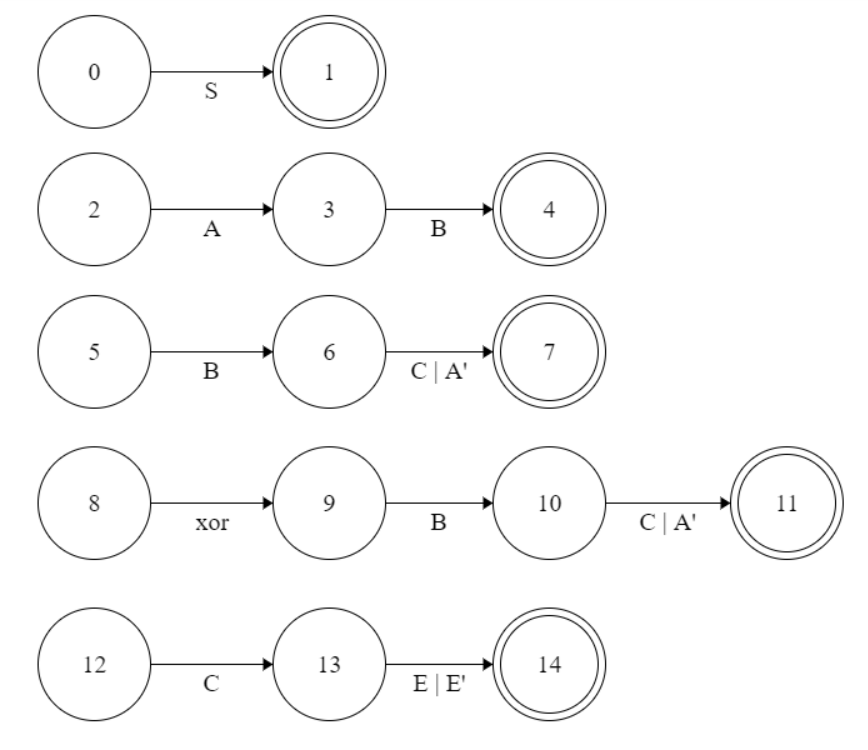
\includegraphics[scale=0.5]{figure/5-2-part1.png}
    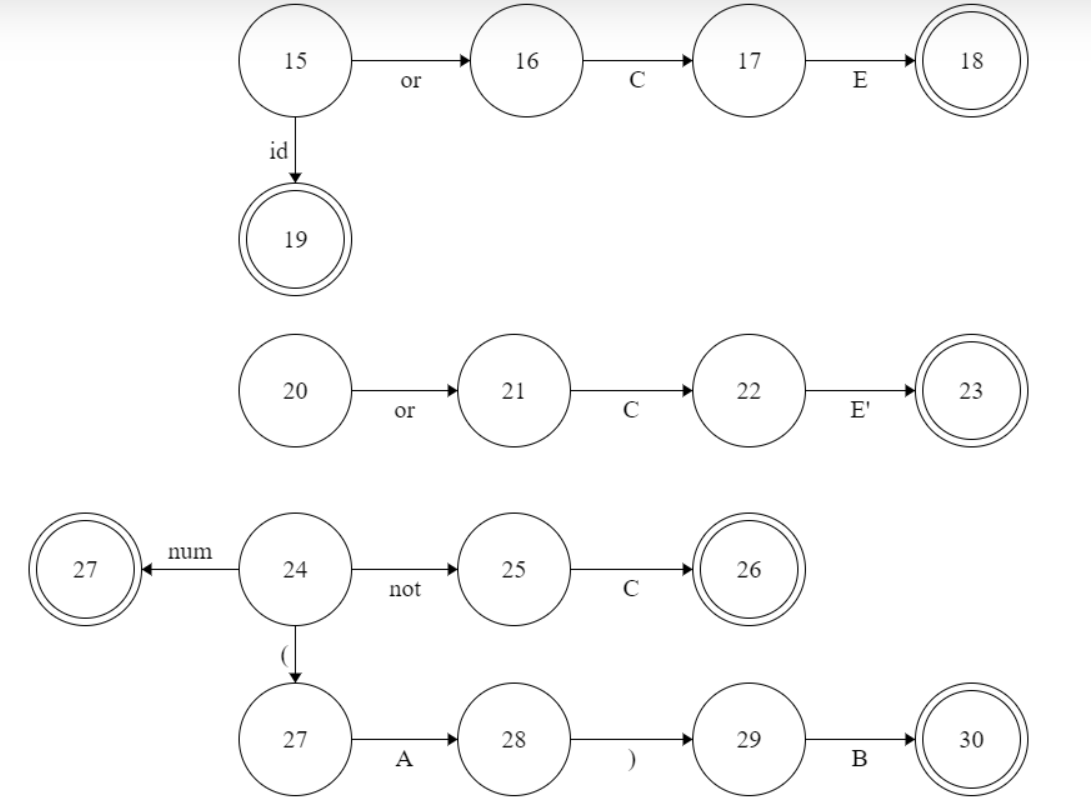
\includegraphics[scale=0.5]{figure/5-2-part2.png}
\end{figure}
سپس شروع به ساده‌سازی می‌کنیم. برای ساده‌سازی بیشتر سعی می‌کنیم که
\lr{transition}ها
را با هم ترکیب بکنیم.
\section*{سوال ششم}
در ابتدا گرامر را می‌نویسیم. همچنین فرض می‌کنیم که
$|$
که در صورت سوال است همان
$-$
است که خیلی قاطی نشود قانون‌ها.
\begin{align*}
    S &\rightarrow G\\
    G &\rightarrow G\&H \big| H \big| G \sim H \big| H \sim I\\
    H &\rightarrow H\#I \big| I \big| H-I\\
    I &\rightarrow (G) \big| id \big| id(I)\\
\end{align*}
مانند همه‌ی سوال‌های دیگر در ابتدا
\lr{First} و \lr{Follow}
هر علامت را پیدا می‌کنیم:
\begin{align*}
    \operatorname{First}(I) &= \{(, id\}\\
    \operatorname{First}(H) &= \{(, id\}\\
    \operatorname{First}(G) &= \{(, id\}\\
    \operatorname{First}(S) &= \{(, id\}\\
    \operatorname{Follow}(S) &= \{\$\}\\
    \operatorname{Follow}(G) &= \{\&, \sim, \$, )\}\\
    \operatorname{Follow}(H) &= \{\&, \sim, \$, ), -, \#\}\\
    \operatorname{Follow}(I) &= \{\&, \sim, \$, ), -, \#\}\\
\end{align*}
حال باید به این موضوع برسیم که چرا این گرامر را نمی‌توان به کمک
\lr{SLR}
پارس کرد. اگر کمی دقت بکنیم متوجه می‌شویم که گرامر اصلا ابهام دارد!
رشته‌ی
$\text{id} \sim \text{id} \sim \text{id}$
را در نظر بگیرید.  در اینجا می‌توان یک
$G$
ساخت و آن را دوبار به کمک
$G \rightarrow G \sim H$
به
$G \sim H \sim H$
رساند یا اینکه در مرحله‌ی دوم بسط دادن آن را مستقیم به
$H \sim I \sim H$
رساند. پس این گرامر ابهام دارد. برای درست کردن آن کافی است که قانون
$G \rightarrow H \sim I$
را حذف کرد چرا که هم
$G$ و $H$ هر دو $H$ و $I$ را \lr{derive}
می‌کنند. در این حالت
\lr{First} و \lr{Follow}ها
عوض نمی‌شوند. حال با این احتساب  جدول
\lr{STL}
را رسم می‌کنیم.
(شکل ممکن است که در چند صفحه بعد باشد)
% https://jsmachines.sourceforge.net/machines/slr.html
% S -> G
% G -> G & H 
% G -> H
% G -> G ~ H
% H -> H # I
% H -> I
% H -> H - I
% I -> ( G )
% I -> id
% I -> id ( I )
\begin{figure}[H]
    \centering
    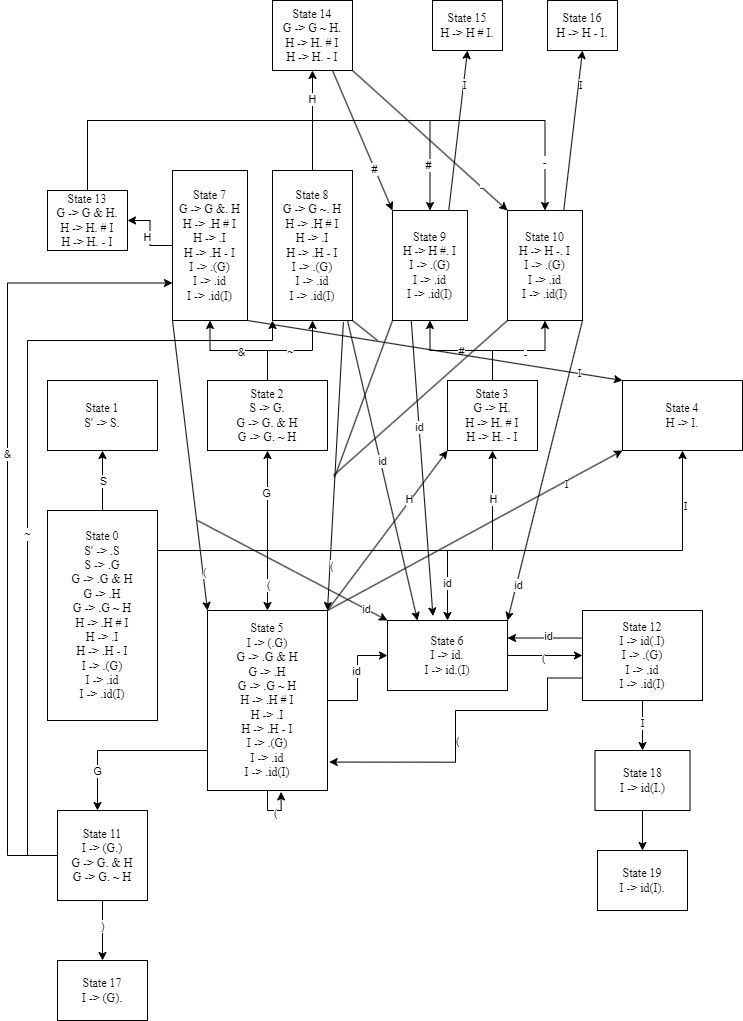
\includegraphics[scale=0.6]{figure/6-table.png}
\end{figure}
حال جدول را با توجه به شکل رسم می‌کنیم:
\begin{align*}
0.&~S' \rightarrow S\\
1.&~S \rightarrow G\\
2.&~G \rightarrow G \& H \\
3.&~G \rightarrow H\\
4.&~G \rightarrow G \sim H\\
5.&~H \rightarrow H \# I\\
6.&~H \rightarrow I\\
7.&~H \rightarrow H - I\\
8.&~I \rightarrow ( G )\\
9.&~I \rightarrow id\\
10.&~I \rightarrow id ( I )\\
\end{align*}
\begin{latin}
    \centering
    \begin{tabular}{|c|c|c|c|c|c|c|c|c|c|c|c|c|c|}
        \hline
        \multirow{2}{*}{State} & \multicolumn{8}{|c|}{Action} & \multicolumn{5}{|c|}{Goto}\\
        \cline{2-14}
        &\&&$\sim$&\#&-&(&)&id&\$&S'&S&G&H&I\\
        \hline
        0& & & & &s5& &s6& & &1&2&3&4\\
        \hline
        1& & & & & & & &acc& & & & & \\
        \hline
        2&s7&s8& & & & & &r1& & & & & \\
        \hline
3&r3&r3&s9&s10& &r3& &r3& & & & & \\
\hline
4&r6&r6&r6&r6& &r6& &r6& & & & & \\
\hline
5& & & & &s5& &s6& & & &11&3&4\\
\hline
6&r9&r9&r9&r9&s12&r9& &r9& & & & & \\
\hline
7& & & & &s5& &s6& & & & &13&4\\
\hline
8& & & & &s5& &s6& & & & &14&4\\
\hline
9& & & & &s5& &s6& & & & & &15\\
\hline
10& & & & &s5& &s6& & & & & &16\\
\hline
11&s7&s8& & & &s17& & & & & & & \\
\hline
12& & & & &s5& &s6& & & & & &18\\
\hline
13&r2&r2&s9&s10& &r2& &r2& & & & & \\
\hline
14&r4&r4&s9&s10& &r4& &r4& & & & & \\
\hline
15&r5&r5&r5&r5& &r5& &r5& & & & & \\
\hline
16&r7&r7&r7&r7& &r7& &r7& & & & & \\
\hline
17&r8&r8&r8&r8& &r8& &r8& & & & & \\
\hline
18& & & & & &s19& & & & & & & \\
\hline
19&r10&r10&r10&r10& &r10& &r10& & & & & \\
\hline
    \end{tabular}
\end{latin}
در نهایت نیز ورودی داده شده را
    \lr{parse}
    می‌کنیم.
    \begin{latin}
        \centering
        \begin{tabular}{c|c|c}
            \textbf{Stack} & \textbf{Buffer} & \textbf{Action}\\
            \hline
            0 & id \& id \# id $\sim$ id\$ & Shift 6\\
            0 id 6 & \& id \# id $\sim$ id\$ & Reduce 9\\
            0 I 4 & \& id \# id $\sim$ id\$ & Reduce 6\\
            0 H 3 & \& id \# id $\sim$ id\$ & Reduce 3\\
            0 G 2 & \& id \# id $\sim$ id\$ & Shift 7\\
            0 G 2 \& 7 & id \# id $\sim$ id\$ & Shift 6\\
            0 G 2 \& 7 id 6 & \# id $\sim$ id\$ & Reduce 9\\
            0 G 2 \& 7 I 4 & \# id $\sim$ id\$ & Reduce 6\\
            0 G 2 \& 7 H 13 & \# id $\sim$ id\$ & Shift 9\\
            0 G 2 \& 7 H 13 \# 9 & id $\sim$ id\$ & Shift 6\\
            0 G 2 \& 7 H 13 \# 9 id 6 & $\sim$ id\$ & Reduce 9\\
            0 G 2 \& 7 H 13 \# 9 I 15 & $\sim$ id\$ & Reduce 5\\
            0 G 2 \& 7 H 13 & $\sim$ id\$ & Reduce 2\\
            0 G 2 & $\sim$ id\$ & Shift 8\\
            0 G 2 $\sim$ 8 & id\$ & Shift 6\\
            0 G 2 $\sim$ 8 id 6 & \$ & Reduce 9\\
            0 G 2 $\sim$ 8 I 4 & \$ & Reduce 6\\
            0 G 2 $\sim$ 8 H 14 & \$ & Reduce 4\\
            0 G 2 & \$ & Reduce 1\\
            0 S 1 & \$ & ACCEPT \\
        \end{tabular}
    \end{latin}
\end{document}
